\section{Chart::Mountain}
\herv{Name:} Chart::Mountain\\ \\
\herv{File:} Mountain.pm\\ \\
\herv{Requires:}Chart::Base, GD, Carp, FileHandle\\ \\
\herv{Description:} \fett{Mountain} is a \fett{subclass} of Chart::Base.\\
The class Mountain creates a mountain chart.\\
\\
\herv{Example:}
\begin{figure}[h]
	\begin{center}
		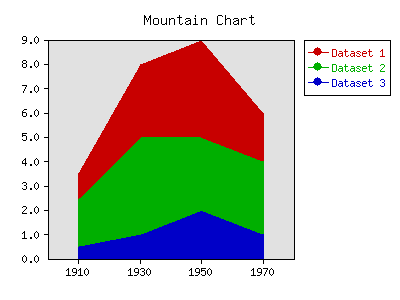
\includegraphics[scale =0.6]{mountain.png}
	\end{center}
	\caption{Mountain chart}
	\label{fig:mountain}
\end{figure}
\begin{verbatim}
use Chart::Mountain;

$g = Chart::Mountain->new();

@data = [ [1910, 1930, 1950, 1970],
          [1, 3, 4, 2],
          [2, 4, 3, 3],
          [0.5, 1, 2, 1]];

$g->set('title' => 'Mountain Chart',
        'grid_lines' => 'false',
        'precision' => 1);

$g->png("mountain.png", @data);

\end{verbatim}
\herv{Constructor:} An instance of a mountain chart object can be created with the constructor new():\\
\fett{\$obj = Chart::Mountain->new();}\\
\fett{\$obj = Chart::Mountain->new(\kursiv{width}, \kursiv{height});}\\
\\
If \fett{new} has no arguments, the constructor returns an image with the size 300x400 pixels. If new has two arguments \kursiv{width} and \kursiv{height}, it returns an image with the desired size. \\ 
\\ 
\herv{Methods:}All universally valid methods, see page \pageref{methods}: Chart::Base. \\
\\
\herv{Attributes/Options:} All universally valid options, see page \pageref{options}. Also available, these special options:
\begin{description}
\item['y\_axes'] Tells chart where to place the y-axis. Valid values are 'left', 'right' and 'both'. Defaults to 'left'.
\end{description}